\documentclass[../../main/thesis_msc.tex]{subfiles}



\begin{document}

	%\chapter{\large Type-Ia Supernovae from non-accreting progenitors}
	\chapter{Results}
	
	%\begin{center}
	%\textbf{Abstract}
	%\end{center}
	
	In this chapter we present the results blah blah
	
	\newpage
	
	\section{Type-Ia Supernovae from non-accreting progenitors}
	
	
		\vspace{3cm}
		
		 \begin{center}
			\textbf{Abstract}
		\end{center}	
		
		some text
		
		\newpage
	
		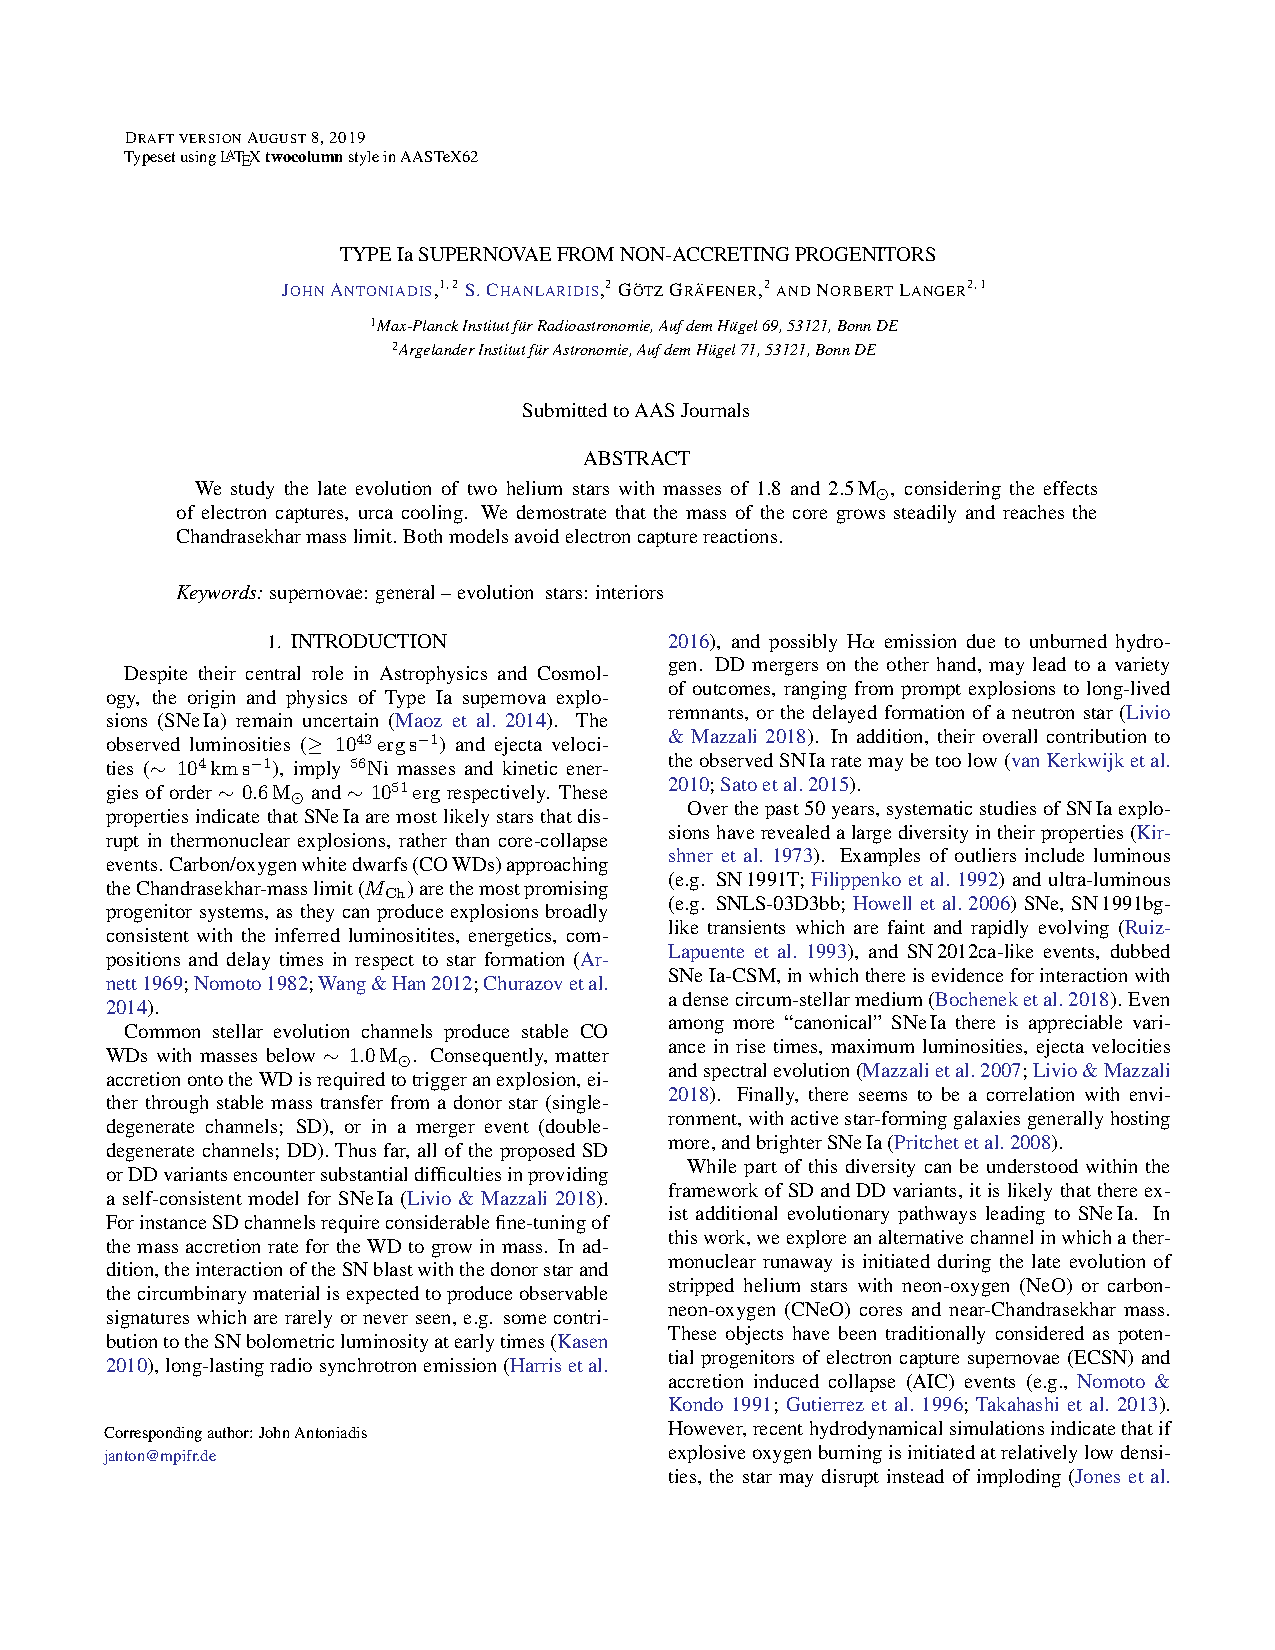
\includepdf[pages=-, scale=1.05, pagecommand={},frame=false, fitpaper=false,
            trim=0mm 0mm -10mm 0mm]{Supernovae.pdf}
            
           
            
            
            
     \section{Helium Stars as Progenitors of Thermonuclear Supernovae}
     
     
    	 \vspace{3cm}
    	 \begin{center}
			\textbf{Abstract}
		\end{center}
		
		
	
Type Ia supernovae (SNe\,Ia) are luminous optical transients characterized by the absence of hydrogen and helium in their spectra. 
The majority of SNe\,Ia are thought to result from the thermonuclear disruption of white dwarfs, which is triggered by mass accretion in a binary system. 
However, both the details of the explosion mechanism and the exact nature of the progenitor systems remain a topic of debate. 
Recent results from wide-field transient surveys, suggest that SNe\,Ia are far more diverse than previously thought.
This diversity could be the result of varied progenitor systems.
We have discovered a novel SN\,Ia progenitor channel, in which a thermonuclear explosion is initiated during the late evolution of stripped helium stars with masses between $\sim 1.8-2.7$\,M$_{\odot}$ which are frequently produced from the mass donors in interacting massive, close binaries. This mechanism does not require accretion from the binary companion and therefore may contribute significantly to the SN\,Ia rate in star-forming galaxies (i.e. at early delay times).

\newpage

     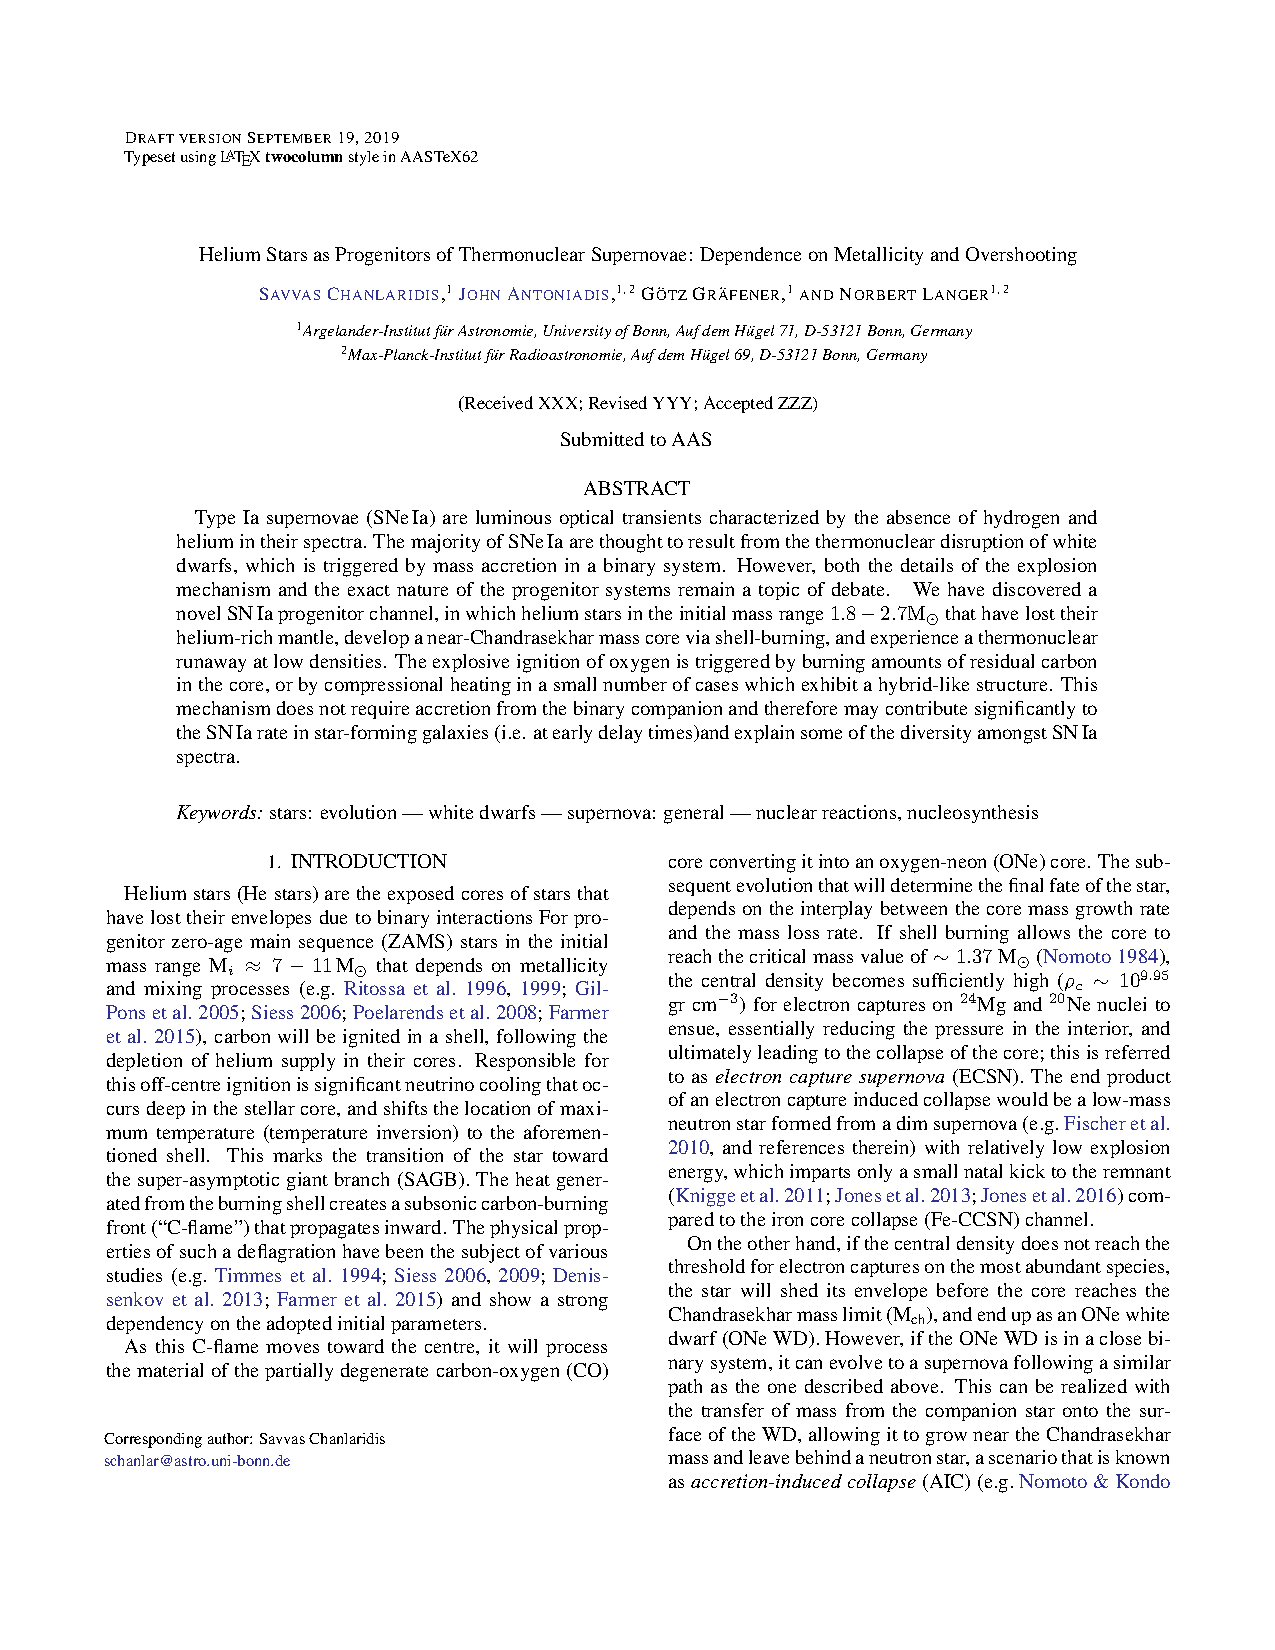
\includepdf[pages=-, scale=1.05, pagecommand={},frame=false, fitpaper=false,
            trim=0mm 0mm -10mm 0mm]{HeliumStars_SNeIa.pdf}
     
	

	
\end{document}